\beginsong{Wir drei, wir geh'n jetzt auf die Walze}[
    wuw={Peter Rohland}, 
    bo={394}, 
    siru={286},
]

\beginverse
\endverse
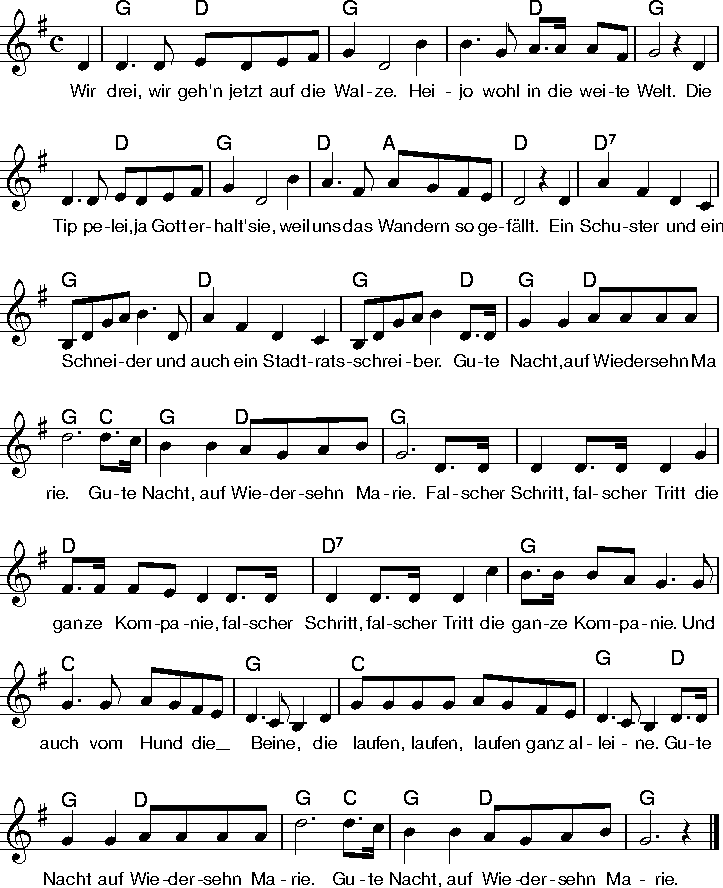
\includegraphics[draft=false, width=1\textwidth]{Noten/Lied098.pdf}

\beginverse
Und \[G]kommen \[D]wir in einen \[G]Flecken, hei-jo, dann \[D]fängt das Fechten \[G]an.
Schnell schultern \[D]wir den Wander\[G]stecken und \[D]klopfen \[A]an bei jeder\[D]mann.
Denn \[D7]hier stehn drei ver\[G]armte, drei \[D]abgebrannte Staats\[G]beamte.
\[D]Gute \[G]Nacht, auf \[D]Wiedersehn Ma\[G]rie, \[C]gute \[G]Nacht, auf \[D]Wiedersehn Ma\[G]rie.
Falscher Schritt, falscher Tritt, die \[D]ganze Kompanie!
Falscher \[D7]Schritt, falscher Tritt, die \[G]ganze Kompanie!
Wir \[C]können nachts nicht ruhig \[G]schlafen, vor \[C]Wanzen, Flöhen und vor Para\[G]graphen.
\[D]Gute \[G]Nacht, auf \[D]Wiedersehn Ma\[G]rie, \[C]gute \[G]Nacht, auf \[D]Wiedersehn Ma\[G]rie.
\endverse

\beginverse
Am ^Rhein, am ^Main und auch am ^Bober, da sieht uns ^manchmal ein Gen^darm.
Schnell krauchen ^wir in einen ^Schober, sonst ^packt er ^uns wohl noch am ^Arm.
Denn ^er schwur stets aufs ^Neue dem ^Staate seine ^Treue.
^Gute ^Nacht, auf ^Wiedersehn Ma^rie, ^gute ^Nacht, auf ^Wiedersehn Ma^rie.
Falscher Schritt, falscher Tritt, die ^ganze Kompanie!
Falscher ^Schritt, falscher Tritt, die ^ganze Kompanie!
Wir ^können nachts nicht ruhig ^schlafen, vor ^Wanzen, Flöhen und vor Para^graphen.
^Gute ^Nacht, auf ^Wiedersehn Ma^rie, ^gute ^Nacht, auf ^Wiedersehn Ma^rie.
\endverse

\beginverse
Und ^blühn am ^Hain die wilden ^Schlehen, dann klopft auch ^mal die Liebe ^an.
Für die, die ^ungern weiter^ziehen, steht ^hie und ^da ein Fenster ^an.
Und ^schlagen früh die ^Finken, dann ^tun wir auch mal ^winken.
^Gute ^Nacht, auf ^Wiedersehn Ma^rie, ^gute ^Nacht, auf ^Wiedersehn Ma^rie. \newpage
Falscher Schritt, falscher Tritt, die ^ganze Kompanie!
Falscher ^Schritt, falscher Tritt, die ^ganze Kompanie!
Be^kanntlich sind die ^Sterne am ^aller- allerschönsten aus der ^Ferne.
^Gute ^Nacht, auf ^Wiedersehn Ma^rie, ^gute ^Nacht, auf ^Wiedersehn Ma^rie,
Ma\[D]rie, Ma\[G]rie!
\endverse

\endsong
